\noindent
\large {\bf Template-Based Decomposition of ChIP-exo Profile Reveals Alternative Binding Configuration Repertoire of Transcription Factors} 


\normalsize 


\noindent \paragraph{Keywords:} 

\noindent \paragraph{Abstract:} 

ChIP-exo is a next generation sequencing technique to
identify genomewide transcription factor (TF) binding
sites in single-nucleotide resolution. Improved from the
predecessor ChIP-seq, ChIP-exo utilizes an exonuclease
to trim off extra 5-prime ends of ChIP DNAs until the
enzyme meets exact binding sites. Thanks to its high resolution sensitivity, ChIP-exo is becoming an increasingly
popular method for delineating previously unseen landscapes of protein-DNA interaction. Most of the computational analysis pipelines for ChIP-exo data so far depend
solely on DNA motif sequences enriched around ChIPexo peaks to identify exact binding sites in high resolution. However, depending on motif information alone is
subject to false positive or false negative errors frequently
(Figure1a), especially because the presence of a specific
motif does not guarantee target protein binding at the locus or a protein can bind to a suboptimal motif in cooperation with other factors.


To overcome this limitation, we propose a template-based
decomposition framework for ChIP-exo data analysis. Our
framework consists of two major parts: 1) optimized motif
mining from ChIP-exo peak-pairs having frequent distances and 2) genomewide template scan of ChIP-exo
signal pattern derived from the motifs (Figure1b). The
basic idea is utilizing ChIP-exo signal at each candidate
binding sites in addition to the motifs. After motif mining
within ChIP-exo peak-pairs having frequent distances, a
template is prepared by aggregating ChIP-exo signal at
high quality motif loci. Then all the random signals from
false-positive binding sites are averaged-out and only real
ChIP-exo signal pattern will be preserved. This template
is used for genomewide scan to identify real binding sites
corresponding to the motif.

We applied our method to interrogate glucocorticoid receptor (GR) binding in vivo, which is an essential factor
for life. From the motif search, we obtained a canonical
GR dimer motif (GRE) from the motif search. First, as a
control analysis, we selected high quality motif loci with p
< 10−4 (Figure1c). Then we prepared a ChIP-exo template
from the GRE motif and did genomewide scan with it.
Remarkably, more than 30\% of the high-quality motif loci
were false positive (Figure1d) even though they were
located within strong ChIP-seq peaks (Figure1e). We also
identified substantial number of dimeric binding at suboptimal motif loci (Figure1d) that were missed when using
motif information only.

Then we selected ChIP-exo peak-pairs that do not match
with the GRE ChIP-exo template (Figure1f-h) for the
next round analysis. From the second motif search, we
obtained HNF6 and FOXA motifs, which were not significantly enriched at the first round. Subsequent template
scans revealed thousands of ChIP-exo signature of HNF6
and FOXA binding (Figure1i-j), which suggests alternative configurations of GR-binding mediated by these lineage factors.
We also successfully applied our method to other ChIPexo datasets, such as estrogen receptor (ER) in a breast
cancer cell line, SOX2 in mouse embryonic stem cell, etc.
The results will be presented at the conference.


Here, we proposed a novel framework for ChIP-exo data
analysis based on a template scan for better accuracy and
robust identification of alternative binding configuration.
There have been many biochemical works to investigate
genomic binding of TFs such as PBM or SELEX. However, our method provide more realistic platform to study
endogenous binding of TFs in vivo, which will extend our
understanding of various repertoire of TF-DNA interactions for gene regulations.

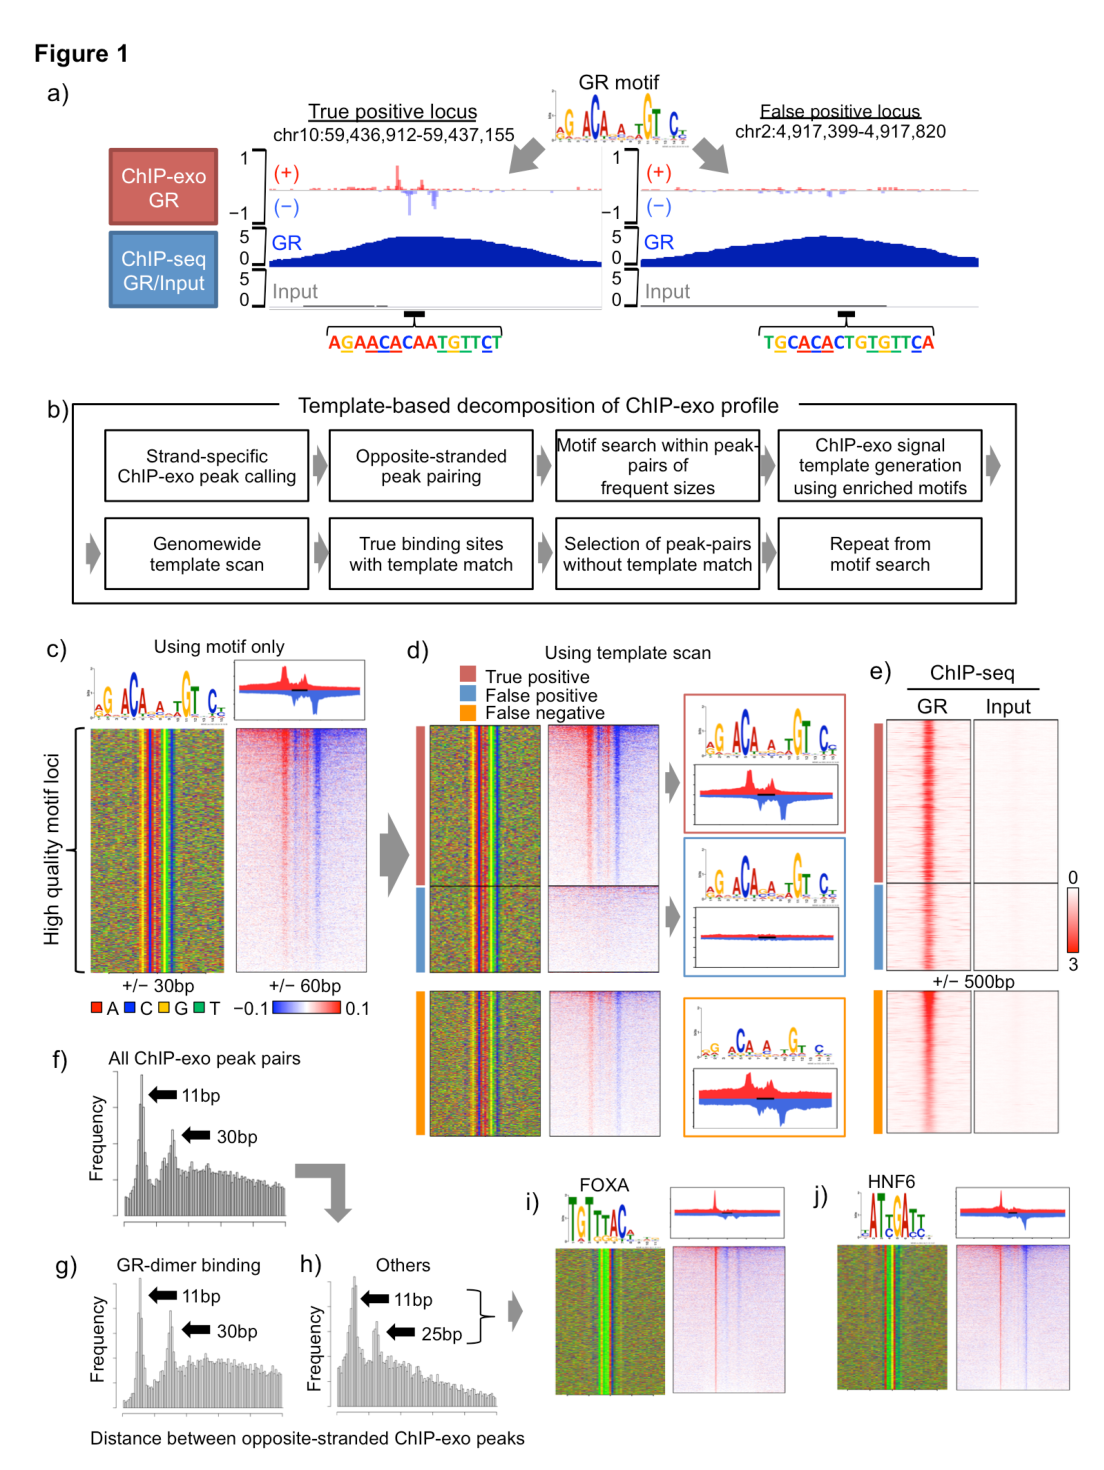
\includegraphics{17.pdf}

\noindent \paragraph{Authors:} 

